\subsection{Evolution of Program Flexibility}
\label{sec:course_pref_evolution}

We begin by showing how {\em Via} recovers high-level, university-wide
trends that have been independently observed in the literature.

We determine the overall {\em flexibility} of departments and their
programs during varying historic time periods. High flexibility means
high ability of students in majors outside the program to include the
program's courses in their curriculum. The measure is thus
complementary to the requirements analysis of
Section~\secref{sec:student-stakeholders} (Figure~\ref{fig:modularity}).

To compute department flexibility for our specific university over
time we use {\em Via} to create separate graphs for generations of
students, separated by their orientation towards engineering, versus
the humanities and social sciences.

We use raw counts of consecutive course enrollments from term to term
to define edge weights between courses. The PageRank execution then
turns those raw counts into transition probabilities.

\begin{figure}
    \centering
    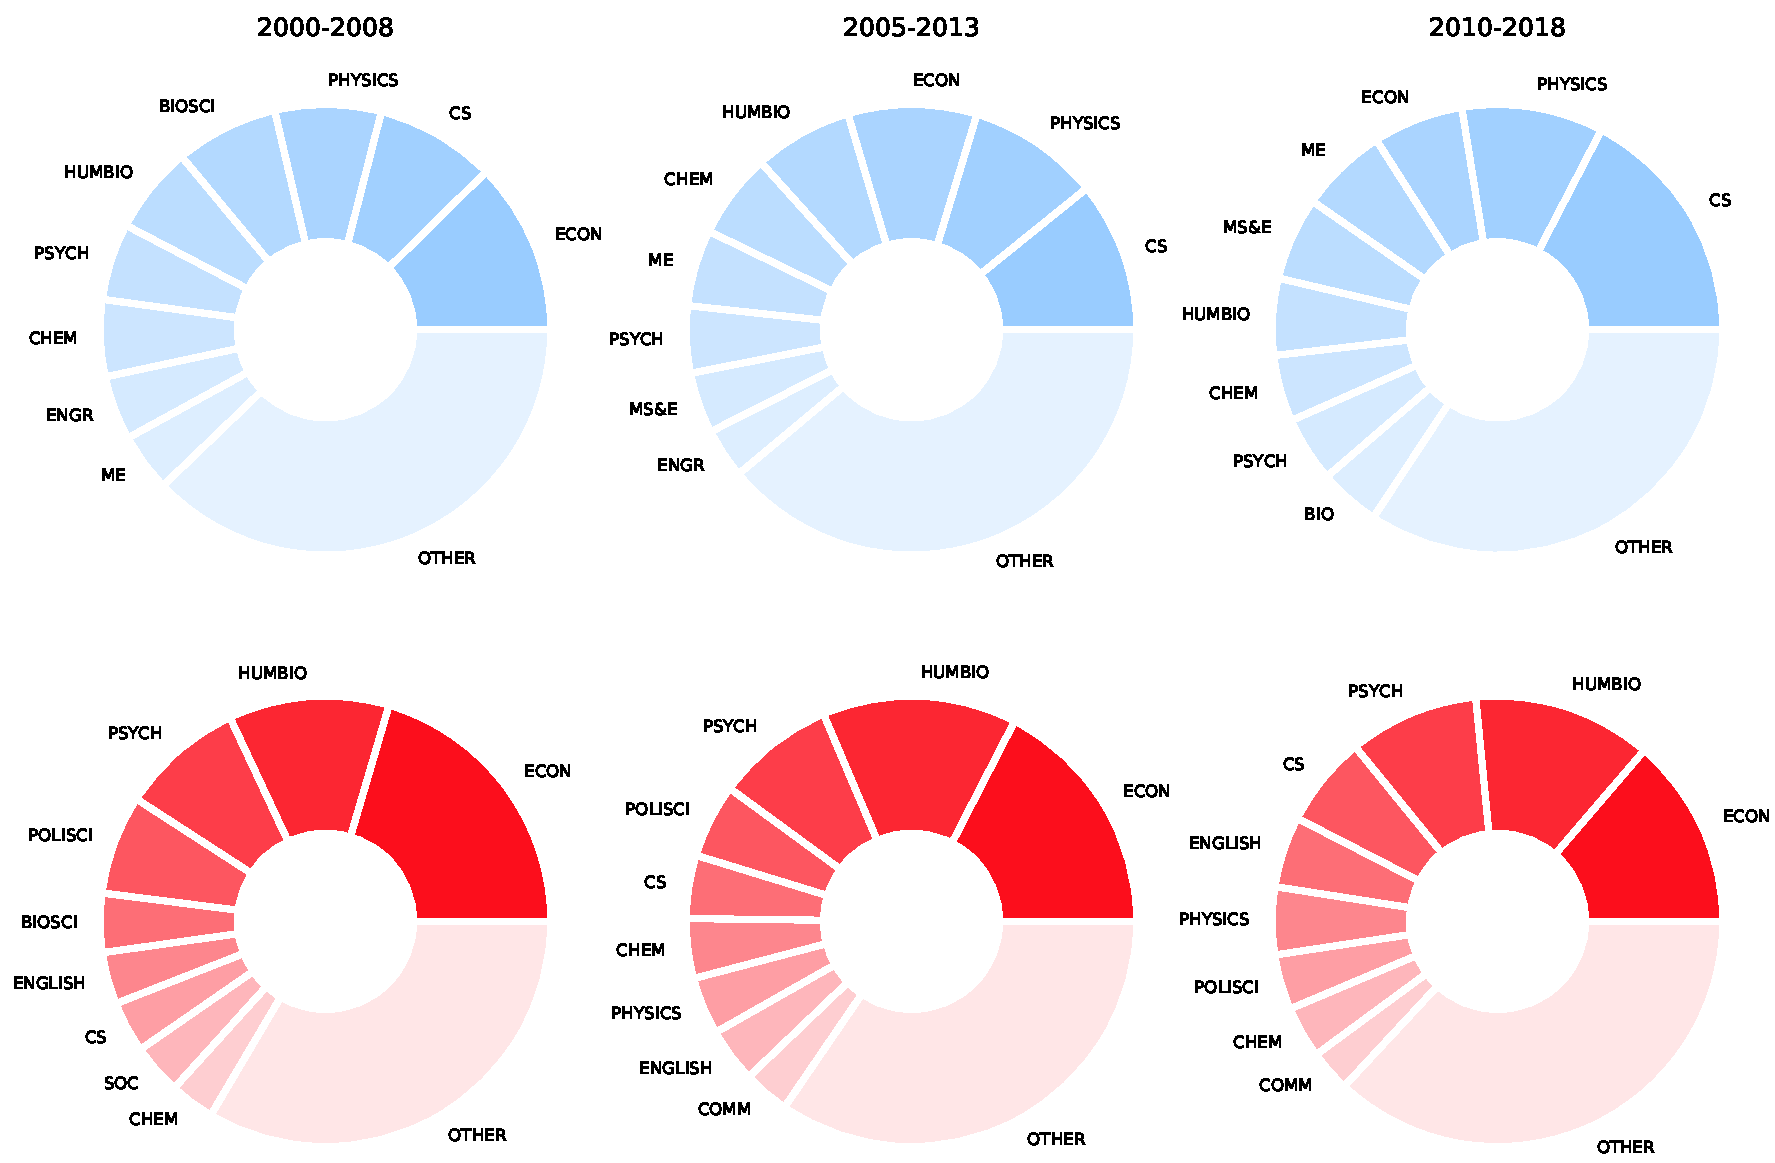
\includegraphics[width=\columnwidth]{Figs/final-evolution.pdf}
    \caption{A comparison over time of PageRank values by department
      in both the entire undergraduate network (top row) and the
      undergraduate network filtered on students who earned a
      Bachelor's of Arts (BA) degree (bottom row).}
    \label{fig:evolution}
\end{figure}

Figure~\ref{fig:evolution} shows the result.

We can interpret the final results as follows: for a given department
$D$ with PageRank score $X$, starting at a random course, and
selecting successors according to successor probability will land
students in $D$ $(X * 100)$\% of the time. Thus, the percentages in
Figure~\ref{fig:evolution} signal the ease with which a department's
courses are available without following a prescribed path.

More generally, we can interpret the relative size of the departments
in Figure~\ref{fig:evolution} as the flexibility of departments across
the different disciplines at the university throughout any time period
in an undergraduate's career.
%% This quantity has an inverse
%% relationship with the activation energy required to begin taking
%% courses in a given department.

%% In this case a department's high PageRank score would indicate a
%% relative ease of entering and taking a course within a particular
%% department.
While closely linked, flexibility differs from metrics of student
composition and enrollments. For example, we see that missing from the
2010-2018 undergraduate results is the mathematics department, despite
it ranking 4th in raw number of enrollments during the given
timeframe. This is likely because students become much less likely to
enroll in math courses after fulfilling the requirement (commonly
during their freshman year), whereas many students enroll in many of
the popular courses in the CS, ECON, and ME departments throughout
their undergraduate career, perhaps because these subjects are less
dependent on knowledge acquired---or not acquired---during the final
years of high school.

We observe that between 2000 and 2018, the PageRank score of the
Computer Science department has increased. This observation applies in
general to all degree-seeking students and to the BA-seeking
students.

Another point to note is a general decrease in accessing economics
courses, but a noticeable uptick in the number of classes taken in
Management Sciences and Engineering (MS\&E). These two trends are
strongly correlated, as the material of MS\&E seeks to combine
economics and finance with computer science and statistics.

Our results are in harmony with observations made by education researchers. Over the past 20 years the proportion of students majoring in STEM, and particularly computer science has varied greatly \cite{ComputingResearchAssociation2017}. Introductory, mid-level and upper-level computer science courses have all shown a demonstrable increase upwards of 150\% of student enrollment between 2000 and 2017. Driving student's decisions to enroll in more technical courses is primarily the greater monetary compensation that these majors promise at the workplace \cite{Downey2007}. Interestingly, however, while the total amount of classes taken within Computer Science has risen noticeably, we do not observe that the total amount of student majors in Computer Science has increased at the same rate. Rather between 2000 and 2010 the number of Computer Science majors showed an uptick of 33\%. However, between 2010 and 2018 the percent increase of Computer Science majors drops to 5.8\%. This finding is more generally in line with the observed trend that the Computer Science major has not experienced a constant exponential increase in popularity. Rather, 2005 was one of the years with the lowest rates of students who self-reported interest in majoring in Computer Science when entering college \cite{Patterson2005}. Between 2000 and 2008 it was, in fact, economics and business-related courses that remained one of the most popular majors of study nation wide \cite{NationalCenterforEducation2018}. Overall, our quantitative analysis is able to corroborate much of the education research regarding course enrollment patterns over the past 20 years. We stress that the methodology used to generate these results is not dependent on the source of data, but is rather facilitated by the graphical modeling of student course enrollments that \textit{Via} enables. In addition, the incorporation of filtering mechanisms beyond time, such as student demographics, would allow for more fine grained understanding of course accessibility based on enrollment data alone.
